\section{14 January 2019}
\begin{defn}
Linear Algebra is the study of vector spaces and the maps between them.
\end{defn}

\begin{defn}
A function $T:V\to W$, from vector space $V$, the domain, to vector space $W$, the codomain, is called a linear transformation if
\[T(c\Vec{u}+\Vec{v})=cT(\Vec{u})+T(\Vec{v});\ \forall \Vec{u},\Vec{v}\in V \wedge c\in \R\]
\end{defn}

\begin{ex}
\[T:\R\to\R;\ T(x)=2x\]
\[T(cu+v) = 2cu + v = cT(u)+T(v)\]
So this is a linear transformation.
\end{ex}
\begin{ex}
\[C^0[0,2\pi] = \{f:[0,2\pi]\to\R\ |\ f\ is \ continuous\}\]
\[S:C^0[0,2\pi]\to \R\]
\[S(f) = f(\pi)\]
Check linearity.
\[S(cf+g) = (cf+g)(\pi)=cf(\pi)+g(\pi)=cS(f)+S(g)\]
\end{ex}

\begin{ex}
\[Let\ T:C^0[0,2\pi]\to \R\]
\[T(f)=\Bar{f}\]
\[T(f)=\frac{1}{2\pi}\int_0^{2\pi}f(x)\ dx\]
Check linearity.
\[T(cf+g)=\frac{1}{2\pi}\int_0^{2\pi}(cf+g)(x)\ dx\]
\[T(cf+g)=\frac{1}{2\pi}(c\int_0^{2\pi}f(x)\ dx+\int_0^{2\pi}g(x)\ dx)\]
\[T(cf+g)=cT(f)+T(g)\]
\end{ex}

$\R^2$ and $\R^3$ are vector spaces, $(x,y)$ is mapped to the vector $\begin{bmatrix}x\\y
\end{bmatrix}$ and $(x,y,z)$ is mapped to the vector $\begin{bmatrix}x\\y\\z
\end{bmatrix}$.
\begin{ex}
Let $T:\R^2\to\R^3$ be defined by \[T(\begin{bmatrix}x\\y\end{bmatrix})=\begin{bmatrix}x+3y\\-x+y\\2x+y\end{bmatrix}\]
Verify linearity.
\[T(c\begin{bmatrix}x\\y\end{bmatrix}+\begin{bmatrix}z\\w\end{bmatrix})=T(\begin{bmatrix}cx+z\\cy+w\end{bmatrix}=\begin{bmatrix}cx+z+3cu+3w\\-cx-z+cy+w\\2cx+2z+cy+w\end{bmatrix}\]
\[T(c\begin{bmatrix}x\\y\end{bmatrix}+\begin{bmatrix}z\\w\end{bmatrix})=\begin{bmatrix}cx+3cu\\-cx+cy\\2cx+cy\end{bmatrix}+\begin{bmatrix}z+3w\\-z+w\\2z+w\end{bmatrix}\]
\[T(c\begin{bmatrix}x\\y\end{bmatrix}+\begin{bmatrix}z\\w\end{bmatrix})=c\begin{bmatrix}x+3u\\-x+y\\2x+y\end{bmatrix}+\begin{bmatrix}z+3w\\-z+w\\2z+w\end{bmatrix}\]
\[T(c\begin{bmatrix}x\\y\end{bmatrix}+\begin{bmatrix}z\\w\end{bmatrix})=cT(\begin{bmatrix}x\\y\end{bmatrix})+T(\begin{bmatrix}z\\w\end{bmatrix})\]
This transformation is the same as the matrix transformation, $\begin{bmatrix}1 & 3\\ -1 & 1\\ -2 & 1\end{bmatrix}$.
\end{ex}

\begin{defn}
Let $T: V\to W$ be a linear transformation. The range or image of $T$ is the is the set range $\mathscr{R}(T)$.
\begin{center}
    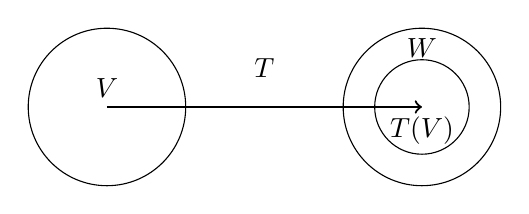
\begin{tikzpicture}
    \draw (1,0) ellipse (1cm and 1cm) node[above] {$V$};
    \draw (5,0) ellipse (1cm and 1cm);
    \draw (5,0.75) node {$W$};
    \draw (3,0.5) node {$T$};
    \draw[thick,->] (1,0) -- (5,0);
    \draw (5,0) ellipse (0.6 cm and 0.6cm) node[below] {$T(V)$};
    \end{tikzpicture}
\end{center}

\end{defn}